\section{Trial Space Selection}
%
Before constructing a ROM, we must first construct a low-dimensional representation of the system state. The simplest method of doing so is constructing the state as a linear combination of a small number of basis vectors, represented by
%
\begin{equation}\label{eq:consSolApprox}
    \begin{aligned}
        \consFunc{\timeVar} \approx \consFuncRom{\timeVar} &\defEq \consVecCent + \sum_{\dummyIdx=1}^{\numConsModes} \consScaleVar_\dummyIdx \consTrialVecIdx \consVarCoefIdx (\timeVar), \\
        &\defEq \consAffineMap(\timeVar),
    \end{aligned}
\end{equation}
%
where $\consVecCent \inROne{\numDOF}$ is a constant translation vector, $\consTrial \defEq \left[\consTrialVec{1},\hdots,\consTrialVec{\numConsModes}\right] \inRTwo{\numDOF}{\numConsModes}$ is the \textit{trial basis}, and $\funcMap{\consVecCoef \defEq \left[\consVarCoef{1}(\timeVar),\hdots,\consVarCoef{\numConsModes}(\timeVar)\right]}{\nonnegReals}{\ROne{\numConsModes}}$ is the \textit{latent state} (alternatively, \textit{modal coefficients} or \textit{generalized coordinates}) vector. The constant diagonal matrix $\consScale \defEq \text{diag}\left(\consScaleVar_1, \hdots , \consScaleVar_{\numDOF}\right) \inRTwo{\numDOF}{\numDOF}$ scales the conservative state variables.

The trial basis spans the affine \textit{trial space}, i.e.,
%
\begin{equation}
    \consTrialSpace \defEq \consVecCent + \textit{Range}\left(\consTrial\right).
\end{equation}
%
It is in this subspace that the approximate solution exists, i.e. $\funcMap{\consVecRom}{\nonnegReals}{\consTrialSpace}$. In reduced-order modeling, we choose $\numConsModes \ll \numDOF$ to generate an extremely compact representation of the state and achieving significant order reduction. The question now becomes \textit{how} we select an appropriate trial space that generates a reasonable approximation of the true state with the lowest dimension $\numConsModes$ as possible. For elliptic and parabolic governing systems, the reduced basis method computes the approximate solution as a linear combination of solution realizations sampled over parameter space. For convection-dominated hyperbolic systems, however, the proper orthogonal decomposition is a more appropriate choice.

\subsection{Proper Orthogonal Decomposition}\label{subsec:POD}
%
The proper orthogonal decomposition (POD) has a long history in a variety of fields under different names, such as the linear Karhunen--Loève approximation in statistics, principal component analysis in data analysis and machine learning, or the Eckart--Young--Mirsky theorem in mathematics. These methods ultimately amount to computing the $\ell^2$-optimal projector of a dataset onto an $\numConsModes$-dimensional subspace. This is formalized by the least-squares problem
%
\begin{equation}\label{eq:podLS}
    \consTrial = \argmin{\dummyMatOne \inRTwo{\numDOF}{\numConsModes}} \norm{ \consDataMatUns - \dummyMatOne \dummyMatOne^\top \consDataMatUns }_\text{F},
\end{equation}
%
where the \textit{data snapshot matrix} is defined as
%
\begin{equation}\label{eq:consSnapMat}
	\consDataMatUns = \left[ \consFuncUns{\initTime}, \; \consFuncUns{\timeVar^1}, \; \hdots \; , \; \consFuncUns{\finalTime} \right] \in \RTwo{\numDOF}{\numSnaps},
\end{equation}
%
and the purely-unsteady component of the solution is given as
%
\begin{equation}\label{eq:consUns}
	\consFuncUns{\timeVar} = \consScaleInv \left[\consFunc{\timeVar} - \consVecCent\right].
\end{equation}
%
The collection of data snapshots defines the \textit{data-driven} nature of this process: a small number of high-fidelity simulations are computed, during which $\numSnaps$ snapshots $\consFunc{\timeVar^{\dummyIdx}}$ of the conservative fields are saved to disk. These snapshots are centered about $\consVecCent$, scaled by $\consScaleInv$, aggregated into the snapshot matrix (Eq.~\ref{eq:consSnapMat}), and the optimal linear projection of this dataset onto an $\numConsModes$-dimensional subspace is computed. Measurements of the quality of this projection, and their use as a diagnostic tool for ROMs of multi-scale, multi-physics systems, are discussed in Section~\ref{subsec:projError}.

The solution of the least-squares problem in Eq.~\ref{eq:podLS} has a convenient analytical solution via the singular value decomposition (SVD). Operating under the assumption that the number of snapshots $\numSnaps$ is less than the number of degrees of freedom $\numDOF$ (true for almost all practical applications), the thin SVD of the data snapshot matrix is given by the form
\begin{equation}\label{eq:svd}
    \consDataMatUns = \leftEvecMat \singVecMat \rightEvecMat^\top,
\end{equation}
where $\leftEvecMat \inRTwo{\numDOF}{\numSnaps}$ and $\rightEvecMat \inRTwo{\numSnaps}{\numSnaps}$ are the left and right singular vectors of $\consDataMatUns$, respectively. The diagonal matrix of singular values $\singValMat = \text{diag}(\singVal_1, \; \singVal_2, \; \hdots, \; \singVal_{\numSnaps}) \inRTwo{\numSnaps}{\numSnaps}$ are ordered such that $\singVal_1 \geq \singVal_2 \geq \hdots \geq \singVal_{\numSnaps} \geq 0 $. The left and right singular vectors are orthonormal, i.e., $\leftEvecMat^T \leftEvecMat = \identMat$ and $\rightEvecMat^T \rightEvecMat = \identMat$. The solution to Eq.~\ref{eq:podLS}, and hence the trial basis $\consTrial$, is computed by extracting the first $\numConsModes$ columns of $\leftEvecMat$, corresponding to the $\numConsModes$ largest singular values. These singular vectors account for the greatest variance in the dataset of any selection of $\numConsModes$ singular vectors.

Algorithms for computing the SVD for extremely large datasets are intensely researched due to the general importance of the SVD in a variety of linear algebra problems. Popular linear algebra packages normally use a process of Householder reflections and QR decompositions, which can be difficult to implement natively in distributed-memory systems. Alternatively, we take particular note of two simpler methods: the method of snapshots, and randomized SVD. All POD bases used to compute ROMs in this thesis utilize the former method, which we detail here briefly. The method of snapshots, pioneered by Sirovich~\cite{Sirovich1987}, begins by recognizing that the right singular vectors of $\consDataMatUns$ are the same as the right eigenvectors of $\consDataMatUns^\top \consDataMatUns \inRTwo{\numSnaps}{\numSnaps}$, whose eigenvalues are also the square of the singular values of $\consDataMatUns$. This can be written as
%
\begin{equation}
	\consDataMatUns^\top \consDataMatUns \rightEvecMat = \singVecMat^2 \rightEvecMat.
\end{equation}
%
As generally $\numSnaps\sim\bigO{100\text{--}1,000}$, and $\consDataMatUns^\top \consDataMatUns$ is symmetric positive definite, this eigenvalue problem can be trivially solved using standard serial routines, such as those supplied by MATLAB, NumPy/SciPy (Python), LAPACK (Fortran), or Eigen (\CC). Leveraging the fact that the right singular vectors are orthonormal, the SVD (Eq.~\ref{eq:svd}) can be rearranged to compute the left singular vectors as
%
\begin{equation}
	\leftEvecMat = \consDataMatUns \rightEvecMat \singVecMat^{-1}.
\end{equation}
%
This approach is notably less memory-intensive than standard SVD routines, and is fairly trivial to implement in a parallel, distributed-memory environment (requiring only a parallel inner product, a serial eigensolve, and local matrix-vector products).

However, even the method of snapshots can be prohibitively memory- and compute-intensive. \textit{Randomized} linear algebra attempts to alleviate much of the computational burden by approximating the SVD by decomposing the action of the data matrix on a small random matrix~\cite{Halko2011}. The number of random samples (columns of the random matrix) increases the accuracy and cost of this approximate solution. Although the randomized SVD is not used for any results in this paper, it would be negligent to not mention its utility for ROMs of large-scale problems. For example, the work by McQuarrie \textit{et al.}~\cite{McQuarrie2021} uses the randomized SVD for decompositions of 2D single-element rocket injector simulation data.


\subsection{Non-linear Autoencoders}\label{subsec:nonlinManifold}

Up until this point we have only discussed linear representations of the solution, of the form given by Eq.~\ref{eq:consSolApprox}. The accuracy of this linear approximation to the subset of solution snapshots is often discussed in terms of the Kolmogorov $n$-width~\cite{Pinkus1985}. We take care to note that the letter $n$ used here has no relation to the time step index used throughout this thesis, but use this notation for consistency with the literature. The Kolmogorov $n$-width is formally defined as
%
\begin{equation}\label{eq:nwidth}
    d_n(\MC{A}) = \underset{\MC{V}_n}{\vphantom{sup}\text{inf}} \enspace \underset{x \in \MC{A}}{\text{sup}} \enspace \underset{y \in \MC{V}_n}{\vphantom{sup}\text{inf}} || x - y ||.
\end{equation}
%
This measures a distance between an \textit{optimal} $n$-dimensional subspace $\MC{V}_n$ and a subset $\MC{A}$ of a normed linear space. Those solution subsets $\MC{A}$ for which increasing $n$ leads to rapidly-improving approximations are said to have a \textit{quickly-decaying} $n$-width. Conversely, those solution subsets which require large $n$ to achieve sufficiently-accurate approximations are said to have a \textit{slowly-decaying} $n$-width. Although computing bounds for $n$-widths is restricted to very specific solution sets, it has been empirically observed that fluid flow fields characterized by convection phenomena and sharp gradients (e.g., shocks or flames) exhibit poor convergence of approximation error via linear representations.

To overcome this inherent challenge, a class of techniques referred to as \textit{non-linear manifold} methods seeks more general and expressive representations of the solution subset. As discussed briefly in Section~\ref{sec:dataDrivenModeling}, kernel principal component analysis~\cite{kernelPCA} and generative topographic mappings~\cite{Bishop1997} are just two traditional methods. In the past two decades, however, with increased access to HPC resources and large datasets, neural networks have become extremely relevant to the dimension-reduction research community.

We take care to note that the following discussion of non-linear autoencoders derives directly from the work by Lee and Carlberg on non-linear manifold projection-based reduced-order models~\cite{Lee2020}. This seminal paper built a strong theoretical foundation for the application of neural network autoencoders in projection-based ROMs, and we find its terminology and notation extremely intuitive. As such, although the results in Chapter~\ref{chap:TransientFlame} expands on this work and provides an honesty evaluation of the cost/benefits tradeoff in neural network PROMs for reacting flows, the credit for developing the method lies solely with Lee and Carlberg. With that said, we begin by providing a very brief primer on neural networks and their relation to dimension-reduction.

\paragraph*{Feedforward Neural Networks}\mbox{}\\
%
From a mathematical point of view, a feedforward neural network can be considered as the successive composition of arbitrary non-linear functions which ingest a vector of input data $\nnInput \inROne{\numNNInput}$ and maps it to a target vector $\nnOutput \inROne{\numNNOutput}$. This process thus takes the form
%
\begin{equation}
	\nnOutput = \nnLayerFunc{\nnInput, \; \nnParams},
\end{equation}
\begin{equation}
	\nnLayerFunc{\nnInput, \; \nnParams} \defEq \nnLayerFuncIdx{\cdot, \; \nnParams^{\numLayers}}{\numLayers} \circ \nnLayerFuncIdx{\cdot, \; \nnParams^{\numLayers-1}}{\numLayers-1} \circ \hdots \circ \nnLayerFuncIdx{\cdot, \; \nnParams^{2}}{2} \circ \nnLayerFuncIdx{\nnInput, \; \nnParams^{1}}{1}.
\end{equation}
%
Each successive function $\funcMap{\nnLayerIdx{\dummyIdx}}{\ROne{N_{\dummyIdx}}}{\ROne{N_{\dummyIdx+1}}}$ is referred to as the $\dummyIdx$th \textit{layer} of the neural network, and $\nnParams \defEq \{\nnParams^{1}, \hdots, \; \nnParams^{\numLayers}\}$ are the parameters which define the layers. The input of the first layer $\nnLayer^1$ is of dimension $\ROne{\numNNInput}$, and the output of the last layer $\nnLayer^{\numLayers}$ is of dimension $\ROne{\numNNOutput}$. All inner input/output dimensions are arbitrary.

As a demonstrative example, one of the simplest forms of $\nnLayer$ is the fully-connected layer, which is given by
%
\begin{equation}
	\nnLayer_{\text{FC}}(\nnInput, \nnParams) \defEq \actFunc{\nnWeights \nnInput + \nnBias}.
\end{equation}
%
The layer parameters are given as the layer weights $\nnWeights \inRTwo{N_{\dummyIdx+1}}{N_{\dummyIdx}}$ and biases $\nnBias \inROne{N_{\dummyIdx+1}}$. The function $\funcMap{\nnAct}{\ROne{N_{\dummyIdx+1}}}{\ROne{N_{\dummyIdx+1}}}$ is a user-specified \textit{activation function}, which is typically chosen to be a non-linear function to supply the non-linear representative power of neural networks. Popular activation functions include sigmoid, tanh, ReLU, and swish functions.

Given a training data set of matching pairs of input vectors and corresponding ``correct'' output vectors (e.g., a picture of a cat and the label ``cat''), the parameters $\nnParams^{\dummyIdx}$ dictate the accuracy of the neural network's attempt to map the input data to the output data. These parameters are computed by an iterative training procedure by which training input is processed by the neural network, a \textit{loss function} $\funcMap{\nnCost}{\ROne{\numNNOutput}}{\mathbb{R}}$ measures how well the network's output matches the correct output vector, and the parameters are updated according to the cost function. This update to the network parameters is typically computed by \textit{gradient descent via backpropagation}, whereby the contribution of a parameter to the loss $\nnCostFunc{\nnOutput, \; \nnLayerFunc{\nnInput, \; \nnParams}}$ determines how it is modified. The mechanics of gradient-based optimization are not described here; the reader is directed to the review by Ruder for further details~\cite{Ruder2016}.

Suffice to say, however, this iterative procedure of measuring the ``correctness'' of the network and incrementally adjusting the parameters can be an incredibly slow and computationally expensive process. Modern GPU and TPU computing architectures have enabled massive acceleration of this training process, but state-of-the-art neural networks have commensurately ballooned in the number of trainable parameters, reaching hundreds of billions~\cite{Brown2020} to trillions of parameters~\cite{Fedus2022} in recent years. Further, gradient descent methods are not guaranteed to find a global optimum, and avoiding inaccurate local optima is an ongoing area of research. Ultimately, this training cost and lack of analytical optimality is the necessary cost of seeking a general, non-linear representation of extremely complex datasets which neural networks target. We now turn to a specific neural network architecture which enables non-linear reduced-order models for fluid flows.

\paragraph{Autoencoder Trial Manifolds}\mbox{}\\
%
Autoencoders describe a specific class of neural networks which are composed of an input network (the \textit{encoder}) which maps the input data to a low-dimensional vector (the \textit{latent state}), followed by an output network (the \textit{decoder}) which attempts to map the latent state back to the input data. That is, the input data and the target output are the same, and the autoencoder learns to compress the data and retrieve it from the low-dimensional representation. In this sense, an autoencoder is trained to learn the identity operation, mapping input data to itself through a low-dimensional bottleneck. A visual representation of a simple autoencoder is shown in Fig.~\ref{fig:aeSample}.
%
\begin{figure}
    \centering
    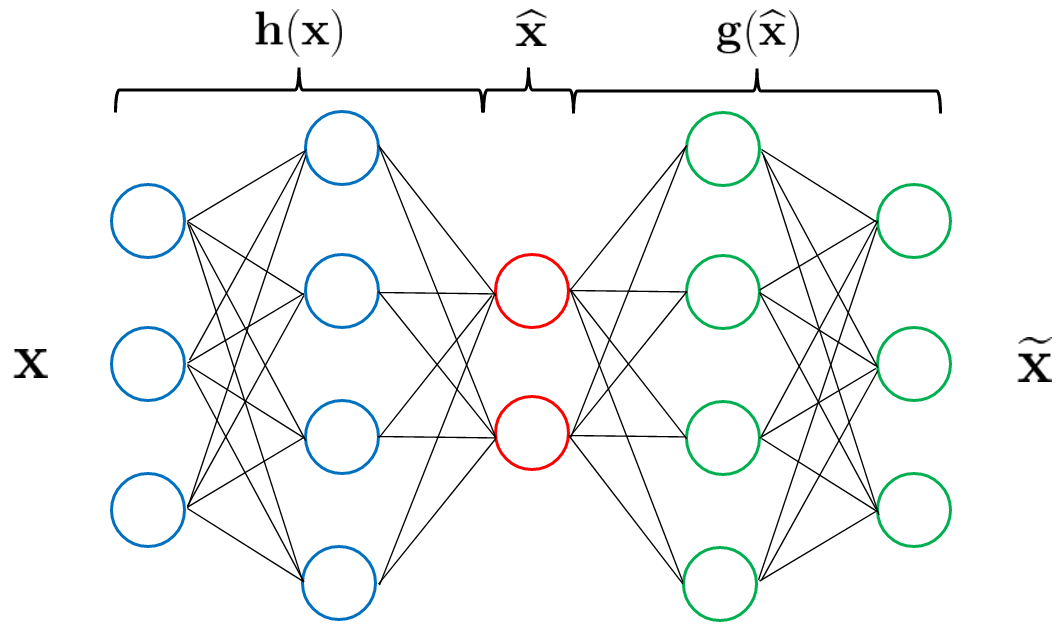
\includegraphics[width=0.75\linewidth]{Chapters/ProjROMs/Images/simpleAE.png}
    \caption{\label{fig:aeSample}Simplified autoencoder composed of encoder network $\encoderFunc{\cdot}$, latent state $\nnInputCoef$, and decoder network $\decoderFunc{\cdot}$, given input $\nnInput$.}
\end{figure}
%
The bottleneck defines the dimension-reduction aspect of autoencoders: the full state may be represented by a low-dimensional state and extracted by the decoder network. However, unlike linear dimension-reduction as provided by POD in Section~\ref{subsec:POD}, neural networks enable arbitrarily non-linear representations of functions with the potential to efficiently approximate solution subsets with slowly-decaying Kolmogorov $n$-widths, such as those observed in convection-dominated fluid flows. For dimension-reduction of fluid flow fields, the training data are the snapshots of the conservative or primitive states. An autoencoder for this data can thus be formalized by the representation
%
\begin{equation}
    \consVecRom = \decoderFunc{\cdot, \nnParams^{\decoderVar}} \circ \encoderFunc{\consVec, \nnParams^{\encoderVar}},
\end{equation}
%
where $\funcMap{\encoder}{\ROne{\numDOF}}{\ROne{\numConsModes}}$ is the encoder network, and $\funcMap{\decoder}{\ROne{\numConsModes}}{\ROne{\numDOF}}$ is the decoder network. We take care to note that the encoder function $\encoder$ is implied to be preceded by a centering and scaling operation, similar to that given in Eq.~\ref{eq:consUns}, and the decoder $\decoder$ is implied to be proceeded by the reverse operation, i.e.
%
\begin{align}
    \encoderFunc{\consVec} &\defEq \nnLayer_{\encoderVar} \left(\consScaleInv\left[\consVec - \consVecCent\right], \nnParams^{\encoderVar}\right), \\
    \decoderFunc{\consVecCoef} &\defEq \consVecCent + \consScale \nnLayer_{\decoderVar} \left(\consVecCoef, \nnParams^{\decoderVar}\right). \label{eq:decoderFunc}
\end{align}
%
Here, $\funcMap{\nnLayer_{\encoderVar}}{\ROne{\numDOF}}{\ROne{\numConsModes}}$ and $\funcMap{\nnLayer_{\decoderVar}}{\ROne{\numConsModes}}{\ROne{\numDOF}}$ are solely the neural network components of the encoder and decoder, respectively. This ensures that the network is trained on standardized data, as was the case for computing the POD basis in Section~\ref{subsec:POD}.

After the autoencoder network is trained as previously detailed, the decoder alone may be extracted, and the physical state may then be approximated as
%
\begin{equation}\label{eq:consSolApproxGen}
    \consVec\left(\timeVar\right) \approx \consVecRom(\timeVar) \defEq \decoderFunc{\consVecCoef\left(\timeVar\right)}.
\end{equation}
%
Note the similarity of Eqs.~\ref{eq:decoderFunc} and~\ref{eq:consSolApproxGen} to the linear representation in Eq.~\ref{eq:consSolApprox}. Indeed, the above form is a more general form of such a low-dimensional representation, and devolves to the linear case when the neural network is replaced by a linear operator, i.e. $\nnLayer_{\decoderVar} \left(\nnInput\right) \defEq \consTrial \nnInput$. Of course, neural networks benefit from supplying arbitrary non-linear representations, and the approximate solution is thus defined on a \textit{non-linear manifold} $\consTrialSpace \defEq \{\decoderFunc{\nnInputCoef} \vert \; \nnInputCoef \inROne{\numConsModes} \}$. In theory, this non-linear manifold has the potential to much more accurately model the true solution subset than a linear subspace for a fixed latent dimension $\numConsModes$. In Chapter~\ref{chap:TransientFlame}, we will show that this is indeed the case given a sufficiently expressive neural network architecture, particularly for solution subsets characterized by propagating waves and sharp gradients.

Moving forward, we will retain the general representation of the approximate state given by Eq.~\ref{eq:consSolApproxGen} in deriving ROMs in Sections~\ref{sec:classicROMs}--\ref{sec:adaptation}. Where appropriate, we will provide simplifications for the case of a linear trial space.
